\documentclass[ignorenonframetext,]{beamer}
\setbeamertemplate{caption}[numbered]
\setbeamertemplate{caption label separator}{: }
\setbeamercolor{caption name}{fg=normal text.fg}
\beamertemplatenavigationsymbolsempty
\usepackage{lmodern}
\usepackage{amssymb,amsmath}
\usepackage{ifxetex,ifluatex}
\usepackage{fixltx2e} % provides \textsubscript
\ifnum 0\ifxetex 1\fi\ifluatex 1\fi=0 % if pdftex
  \usepackage[T1]{fontenc}
  \usepackage[utf8]{inputenc}
\else % if luatex or xelatex
  \ifxetex
    \usepackage{mathspec}
  \else
    \usepackage{fontspec}
  \fi
  \defaultfontfeatures{Ligatures=TeX,Scale=MatchLowercase}
\fi
\usefonttheme{structurebold}
% use upquote if available, for straight quotes in verbatim environments
\IfFileExists{upquote.sty}{\usepackage{upquote}}{}
% use microtype if available
\IfFileExists{microtype.sty}{%
\usepackage{microtype}
\UseMicrotypeSet[protrusion]{basicmath} % disable protrusion for tt fonts
}{}
\newif\ifbibliography
\usepackage{color}
\usepackage{fancyvrb}
\newcommand{\VerbBar}{|}
\newcommand{\VERB}{\Verb[commandchars=\\\{\}]}
\DefineVerbatimEnvironment{Highlighting}{Verbatim}{commandchars=\\\{\}}
% Add ',fontsize=\small' for more characters per line
\usepackage{framed}
\definecolor{shadecolor}{RGB}{248,248,248}
\newenvironment{Shaded}{\begin{snugshade}}{\end{snugshade}}
\newcommand{\KeywordTok}[1]{\textcolor[rgb]{0.13,0.29,0.53}{\textbf{{#1}}}}
\newcommand{\DataTypeTok}[1]{\textcolor[rgb]{0.13,0.29,0.53}{{#1}}}
\newcommand{\DecValTok}[1]{\textcolor[rgb]{0.00,0.00,0.81}{{#1}}}
\newcommand{\BaseNTok}[1]{\textcolor[rgb]{0.00,0.00,0.81}{{#1}}}
\newcommand{\FloatTok}[1]{\textcolor[rgb]{0.00,0.00,0.81}{{#1}}}
\newcommand{\ConstantTok}[1]{\textcolor[rgb]{0.00,0.00,0.00}{{#1}}}
\newcommand{\CharTok}[1]{\textcolor[rgb]{0.31,0.60,0.02}{{#1}}}
\newcommand{\SpecialCharTok}[1]{\textcolor[rgb]{0.00,0.00,0.00}{{#1}}}
\newcommand{\StringTok}[1]{\textcolor[rgb]{0.31,0.60,0.02}{{#1}}}
\newcommand{\VerbatimStringTok}[1]{\textcolor[rgb]{0.31,0.60,0.02}{{#1}}}
\newcommand{\SpecialStringTok}[1]{\textcolor[rgb]{0.31,0.60,0.02}{{#1}}}
\newcommand{\ImportTok}[1]{{#1}}
\newcommand{\CommentTok}[1]{\textcolor[rgb]{0.56,0.35,0.01}{\textit{{#1}}}}
\newcommand{\DocumentationTok}[1]{\textcolor[rgb]{0.56,0.35,0.01}{\textbf{\textit{{#1}}}}}
\newcommand{\AnnotationTok}[1]{\textcolor[rgb]{0.56,0.35,0.01}{\textbf{\textit{{#1}}}}}
\newcommand{\CommentVarTok}[1]{\textcolor[rgb]{0.56,0.35,0.01}{\textbf{\textit{{#1}}}}}
\newcommand{\OtherTok}[1]{\textcolor[rgb]{0.56,0.35,0.01}{{#1}}}
\newcommand{\FunctionTok}[1]{\textcolor[rgb]{0.00,0.00,0.00}{{#1}}}
\newcommand{\VariableTok}[1]{\textcolor[rgb]{0.00,0.00,0.00}{{#1}}}
\newcommand{\ControlFlowTok}[1]{\textcolor[rgb]{0.13,0.29,0.53}{\textbf{{#1}}}}
\newcommand{\OperatorTok}[1]{\textcolor[rgb]{0.81,0.36,0.00}{\textbf{{#1}}}}
\newcommand{\BuiltInTok}[1]{{#1}}
\newcommand{\ExtensionTok}[1]{{#1}}
\newcommand{\PreprocessorTok}[1]{\textcolor[rgb]{0.56,0.35,0.01}{\textit{{#1}}}}
\newcommand{\AttributeTok}[1]{\textcolor[rgb]{0.77,0.63,0.00}{{#1}}}
\newcommand{\RegionMarkerTok}[1]{{#1}}
\newcommand{\InformationTok}[1]{\textcolor[rgb]{0.56,0.35,0.01}{\textbf{\textit{{#1}}}}}
\newcommand{\WarningTok}[1]{\textcolor[rgb]{0.56,0.35,0.01}{\textbf{\textit{{#1}}}}}
\newcommand{\AlertTok}[1]{\textcolor[rgb]{0.94,0.16,0.16}{{#1}}}
\newcommand{\ErrorTok}[1]{\textcolor[rgb]{0.64,0.00,0.00}{\textbf{{#1}}}}
\newcommand{\NormalTok}[1]{{#1}}
\usepackage{graphicx,grffile}
\makeatletter
\def\maxwidth{\ifdim\Gin@nat@width>\linewidth\linewidth\else\Gin@nat@width\fi}
\def\maxheight{\ifdim\Gin@nat@height>\textheight0.8\textheight\else\Gin@nat@height\fi}
\makeatother
% Scale images if necessary, so that they will not overflow the page
% margins by default, and it is still possible to overwrite the defaults
% using explicit options in \includegraphics[width, height, ...]{}
\setkeys{Gin}{width=\maxwidth,height=\maxheight,keepaspectratio}

% Prevent slide breaks in the middle of a paragraph:
\widowpenalties 1 10000
\raggedbottom

\AtBeginPart{
  \let\insertpartnumber\relax
  \let\partname\relax
  \frame{\partpage}
}
\AtBeginSection{
  \ifbibliography
  \else
    \let\insertsectionnumber\relax
    \let\sectionname\relax
    \frame{\sectionpage}
  \fi
}
\AtBeginSubsection{
  \let\insertsubsectionnumber\relax
  \let\subsectionname\relax
  \frame{\subsectionpage}
}

\setlength{\emergencystretch}{3em}  % prevent overfull lines
\providecommand{\tightlist}{%
  \setlength{\itemsep}{0pt}\setlength{\parskip}{0pt}}
\setcounter{secnumdepth}{0}
\definecolor{links}{HTML}{800080}
\hypersetup{colorlinks,linkcolor=,urlcolor=links}

\title{Web Data Collection with R}
\subtitle{JavaScript Case Study}
\author{Peter Meißner / 2016-02-29 -- 2016-03-04 / ECPR WSMT}
\date{}

\begin{document}
\frame{\titlepage}

\begin{frame}
\tableofcontents[hideallsubsections]
\end{frame}

\section{The Queens Christmas
Speeches}\label{the-queens-christmas-speeches}

\begin{frame}{Teaser}

\begin{itemize}
\tightlist
\item
  god ssave the queen
\end{itemize}

\end{frame}

\begin{frame}[fragile]{some preparations}

\begin{Shaded}
\begin{Highlighting}[]
\KeywordTok{require}\NormalTok{(stringr)}
\KeywordTok{require}\NormalTok{(RSelenium)}
\KeywordTok{require}\NormalTok{(rvest)}
\KeywordTok{require}\NormalTok{(wordcloud)}
\end{Highlighting}
\end{Shaded}

\end{frame}

\begin{frame}[fragile]{some preparations}

\begin{Shaded}
\begin{Highlighting}[]
\NormalTok{url1 <-}\StringTok{ "http://www.royal.gov.uk/ImagesandBroadcasts"}
\NormalTok{url2 <-}\StringTok{ "/TheQueensChristmasBroadcasts/ChristmasBroadcasts"}
\NormalTok{url3 <-}\StringTok{ "/ChristmasBroadcast"}
\NormalTok{base_url <-}\StringTok{ }\KeywordTok{str_c}\NormalTok{(url1, url2, url3)}

\CommentTok{# make directory to save files in }
\KeywordTok{dir.create}\NormalTok{(}\StringTok{"Queens_Speeches"}\NormalTok{, }\DataTypeTok{showWarnings =} \NormalTok{F)}
\end{Highlighting}
\end{Shaded}

\end{frame}

\begin{frame}[fragile]{starting up engines}

\begin{Shaded}
\begin{Highlighting}[]
\KeywordTok{checkForServer}\NormalTok{() }\CommentTok{# search for and download Selenium Server java binary.  Only need to run once.}
\CommentTok{# linux: https://christopher.su/2015/selenium-chromedriver-ubuntu/}
\CommentTok{# windows: make sure to use Java 64bit for R 64Bit !!!}
\end{Highlighting}
\end{Shaded}

\end{frame}

\begin{frame}[fragile]{starting up engines}

\begin{Shaded}
\begin{Highlighting}[]
\KeywordTok{startServer}\NormalTok{() }\CommentTok{# run Selenium Server binary}
\NormalTok{remDr <-}\StringTok{ }\KeywordTok{remoteDriver}\NormalTok{(}\DataTypeTok{browserName=}\StringTok{"chrome"}\NormalTok{, }\DataTypeTok{port=}\DecValTok{4444}\NormalTok{)}
\NormalTok{remDr$}\KeywordTok{open}\NormalTok{()}
\NormalTok{remDr$}\KeywordTok{navigate}\NormalTok{(}\StringTok{"http://www.royal.gov.uk/"}\NormalTok{) }

\NormalTok{?remoteDriver}
\end{Highlighting}
\end{Shaded}

\end{frame}

\begin{frame}[fragile]{screen shot}

\begin{Shaded}
\begin{Highlighting}[]
\NormalTok{remDr$}\KeywordTok{screenshot}\NormalTok{(}\DataTypeTok{display =} \NormalTok{F, }
                 \DataTypeTok{useViewer=}\NormalTok{F, }
                 \DataTypeTok{file=}\StringTok{"screen1.png"}\NormalTok{)}
\end{Highlighting}
\end{Shaded}

\end{frame}

\begin{frame}{screen shot}

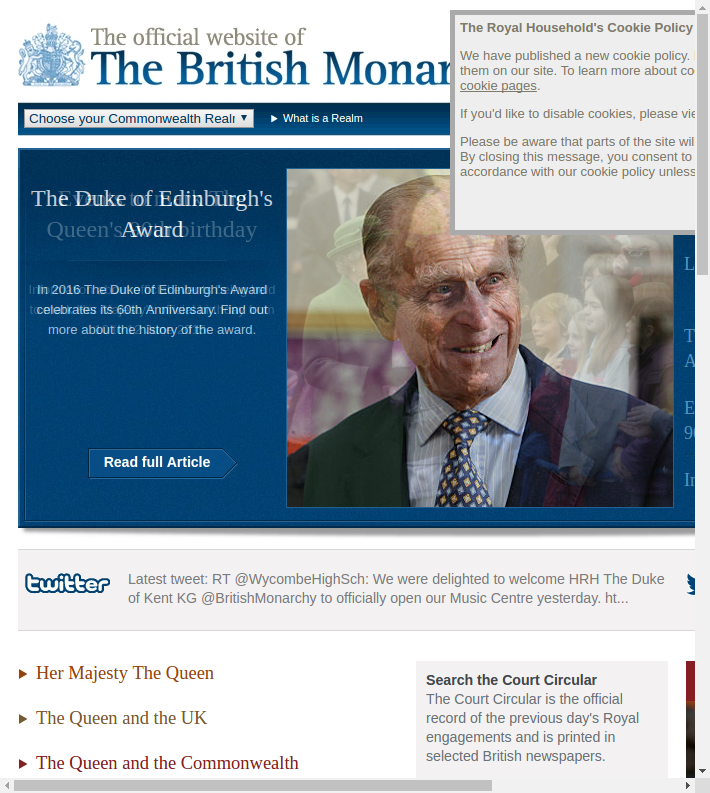
\includegraphics{screen1.png}

\end{frame}

\begin{frame}[fragile]{getting speeches}

\begin{Shaded}
\begin{Highlighting}[]
\NormalTok{for(i in }\DecValTok{1953}\NormalTok{:}\DecValTok{2015}\NormalTok{)\{}
  \NormalTok{url <-}\StringTok{ }\KeywordTok{str_c}\NormalTok{(base_url, i, }\StringTok{".aspx"}\NormalTok{)}
  \NormalTok{remDr$}\KeywordTok{navigate}\NormalTok{(url)   }
  
  \NormalTok{html   <-}\StringTok{ }\NormalTok{remDr$}\KeywordTok{getPageSource}\NormalTok{()[[}\DecValTok{1}\NormalTok{]]}
  \NormalTok{parsed <-}\StringTok{ }\KeywordTok{htmlParse}\NormalTok{(html)}
  \NormalTok{speech <-}\StringTok{ }\KeywordTok{xpathSApply}\NormalTok{(parsed, }
                        \StringTok{'//div[@id="content"]/p'}\NormalTok{, }
                        \NormalTok{xmlValue)}
  \NormalTok{speech_short <-}\StringTok{ }\NormalTok{speech[}\DecValTok{2}\NormalTok{:}\KeywordTok{length}\NormalTok{(speech)]}
  \KeywordTok{write}\NormalTok{(speech_short, }\KeywordTok{str_c}\NormalTok{(}\StringTok{"Queens_Speeches/"}\NormalTok{, i, }\StringTok{".txt"}\NormalTok{))}
\NormalTok{\}}
\end{Highlighting}
\end{Shaded}

\end{frame}

\begin{frame}[fragile]{text}

\begin{Shaded}
\begin{Highlighting}[]
\NormalTok{text  <-}\StringTok{ }\KeywordTok{str_c}\NormalTok{(}\KeywordTok{readLines}\NormalTok{(}\StringTok{"Queens_Speeches/2014.txt"}\NormalTok{),}
               \DataTypeTok{collapse=}\StringTok{"}\CharTok{\textbackslash{}n}\StringTok{"}\NormalTok{)}
\KeywordTok{substring}\NormalTok{(text, }\DecValTok{1}\NormalTok{, }\DecValTok{150}\NormalTok{)}
\end{Highlighting}
\end{Shaded}

\begin{verbatim}
## [1] "In the ruins of the old Coventry Cathedral is a sculpture of a man and a woman reaching out to embrace each other. The sculptor was inspired by the st"
\end{verbatim}

\end{frame}

\begin{frame}[fragile]{some cleansing}

\begin{Shaded}
\begin{Highlighting}[]
\KeywordTok{library}\NormalTok{(tm)}
\NormalTok{corpus <-}\StringTok{ }\KeywordTok{tolower}\NormalTok{(text)}
\NormalTok{corpus <-}\StringTok{ }\KeywordTok{removeNumbers}\NormalTok{(corpus)}
\NormalTok{corpus <-}\StringTok{ }\KeywordTok{removeWords}\NormalTok{(corpus, }\KeywordTok{stopwords}\NormalTok{(}\StringTok{'english'}\NormalTok{))}
\NormalTok{corpus <-}\StringTok{ }\KeywordTok{stemDocument}\NormalTok{(corpus)}
\end{Highlighting}
\end{Shaded}

\end{frame}

\begin{frame}[fragile]{word frequencies}

\begin{Shaded}
\begin{Highlighting}[]
\NormalTok{words <-}\StringTok{ }\KeywordTok{unlist}\NormalTok{(}\KeywordTok{str_split}\NormalTok{(corpus, }\StringTok{"}\CharTok{\textbackslash{}\textbackslash{}}\StringTok{W"}\NormalTok{))}
\NormalTok{words <-}\StringTok{ }\NormalTok{words[words!=}\StringTok{""} \NormalTok{&}\StringTok{ }\NormalTok{words!=}\StringTok{" "}\NormalTok{]}
\KeywordTok{tail}\NormalTok{(}\KeywordTok{sort}\NormalTok{(}\KeywordTok{table}\NormalTok{(words)),}\DecValTok{10}\NormalTok{)}
\end{Highlighting}
\end{Shaded}

\begin{verbatim}
## words
##      sculpture          still             us         people          today 
##              3              3              3              4              4 
##          truce          games reconciliation            war      christmas 
##              4              5              7              7              8
\end{verbatim}

\end{frame}

\begin{frame}[fragile]{wordclouds}

\begin{Shaded}
\begin{Highlighting}[]
\NormalTok{colors <-}\StringTok{ }\KeywordTok{c}\NormalTok{(}\StringTok{"#CD8B34"}\NormalTok{, }\StringTok{"#89B151"}\NormalTok{, }\StringTok{"#01ABE9"}\NormalTok{, }
            \StringTok{"#1B346C"}\NormalTok{, }\StringTok{"#F54B1A"}\NormalTok{, }\StringTok{"#4B574D"}\NormalTok{,}
            \StringTok{"#609F80"}\NormalTok{, }\StringTok{"#AF420A"}\NormalTok{, }\StringTok{"#D67236"}\NormalTok{,}
            \StringTok{"#FD6467"}\NormalTok{)}
\KeywordTok{wordcloud}\NormalTok{(words, }\DataTypeTok{colors=}\NormalTok{colors)}
\end{Highlighting}
\end{Shaded}

\end{frame}

\begin{frame}{wordclouds}

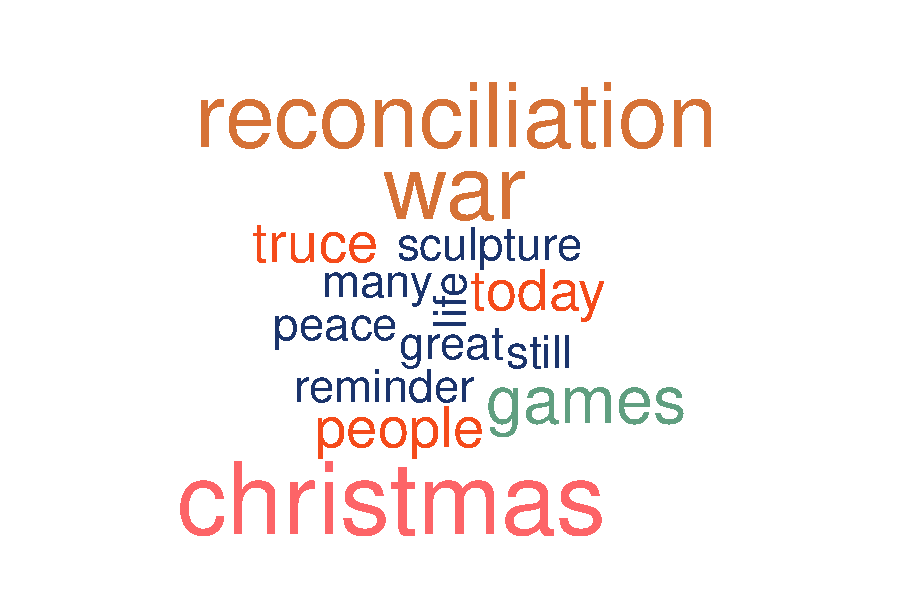
\includegraphics{wc1999.pdf}

\end{frame}

\begin{frame}{RSelenium alternative}

\begin{itemize}
\tightlist
\item
  rdom / phantom.js
\item
  \url{https://github.com/cpsievert/rdom}
\end{itemize}

\end{frame}

\begin{frame}{Live Clicking // Remote Building}

\end{frame}

\end{document}
